\setcounter{section}{0}
\part{Wissensrepräsentation und lineare kontinuierliche Systeme}
\section{Lineare kontinuierliche Systeme}
\subsection{}
\textbf{Welche Annahmen liegen dem linearen Einspurmodell zugrunde? Nennen Sie mindestens 5 Stück.}
\begin{itemize}
    \item Reduktion auf ein Rad pro Achse, d.h. $s_l=s_r=0;\ c_{\alpha}=c_{\alpha,l}+c_{\alpha_r}$
    \item Gesamte Masse im Schwerpunkt
    \item Schwerpunkt auf Höhe der Fahrbahn (damit Betrachtung von Wank-, Nick-, und Hubbewegung wegfällt)
    \item Konstante Fahrzeuggeschwindigkeit
    \item Kleine Winkel ($\sin x=x, \cos x=1, \tan x=x$)
    \item Keine Radlastschwankungen
    \item Zwei Systemzustände (Gierrate $\dot{\psi}$, Schwimmwinekl $\beta$)
    \item Lineare Reifenkennlinie
    \item Reine Vorderachslenkung $\delta_H=0$
    \item Gültig bis ca. $|a_y|\leq4\dfrac{m}{s^2}$
\end{itemize}

\subsection{}
\textbf{Zeichnen Sie ein Blockschaltbild eines dynamischen Systems mit Beobachter. Beschriften Sie das Blockschaltbild sorgfältig.}
\begin{figure}[H]
    \centering
    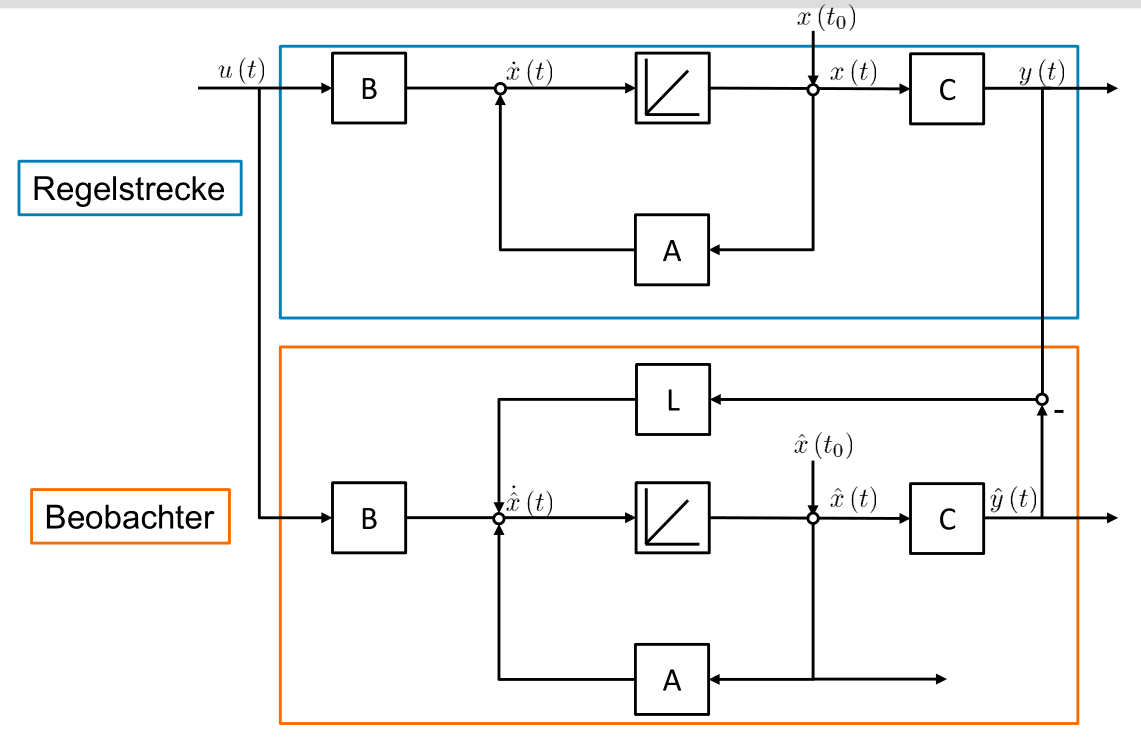
\includegraphics[width=.5\linewidth]{Graphics/beobrachter_blockbild.png}
\end{figure}
\subsection{}
\textbf{Reduzieren Sie das gegebene Querführungsmodell 5.Ordnung soweit wie möglich, so dass damit ein Schwimmwinkelbeobachter konstruierbar ist. Notieren Sie das Modell in Zustandsdarstellung unter der Annahme, dass der Lenkwinkel die einzige Eingangsgröße ist.}

\begin{equation}
    \left(
    \begin{array}{c}
            \dot{\lambda}    \\
            \ddot{\Psi_V}    \\
            \dot{\beta}      \\
            \dot{\Psi_{rel}} \\
            \dot{y}          \\
        \end{array}
    \right)=
    \left(
    \begin{array}{ccccc}
            0                                & 0                                                        & 0                                                   & 0 & 0 \\
            \dfrac{c_{\alpha v}l_{v}}{I_{z}} & -\dfrac{c_{\alpha v}l_{v}^2+c_{\alpha h}l_{h}^2}{I_{z}v} & -\dfrac{c_{\alpha v}l_{v}-c_{\alpha h}l_{h}}{I_{z}} & 0 & 0 \\
            \dfrac{c_{\alpha v}}{mv}         & -1-\dfrac{c_{\alpha v}l_{v}-c_{\alpha h}l_{h}}{mv^2}     & -\dfrac{c_{\alpha v}+c_{\alpha h}}{mv}              & 0 & 0 \\
            0                                & 1                                                        & 0                                                   & 0 & 0 \\
            0                                & 0                                                        & v                                                   & v & 0 \\
        \end{array}
    \right)
    \left(
    \begin{array}{c}
            \lambda      \\
            \dot{\Psi_V} \\
            \beta        \\
            \Psi_{rel}   \\
            y            \\
        \end{array}
    \right)+
    \left(
    \begin{array}{c}
            1 \\
            0 \\
            0 \\
            0 \\
            0 \\
        \end{array}
    \right)\dot{\lambda}+
    \left(
    \begin{array}{c}
            0  \\
            0  \\
            0  \\
            -v \\
            0  \\
        \end{array}
    \right)c_0
\end{equation}

\begin{equation}
    \left(
    \begin{array}{c}
        \ddot{\Psi_V} \\
        \dot{\beta}   \\
    \end{array}
    \right)=
    \left(
    \begin{array}{cc}
        -\dfrac{c_{\alpha v}l_{v}^2+c_{\alpha h}l_{h}^2}{I_{z}v} & -\dfrac{c_{\alpha v}l_{v}-c_{\alpha h}l_{h}}{I_{z}} \\
        -1-\dfrac{c_{\alpha v}l_{v}-c_{\alpha h}l_{h}}{mv^2}     & -\dfrac{c_{\alpha v}+c_{\alpha h}}{mv}              \\
    \end{array}
    \right)
    \left(
    \begin{array}{c}
        \dot{\Psi_V} \\
        \beta        \\
    \end{array}
    \right)+
    \left(
    \begin{array}{c}
        \dfrac{c_{\alpha v}l_v}{I_{Z}} \\
        \dfrac{c_{\alpha v}}{mv}       \\
    \end{array}
    \right)\lambda
\end{equation}

\subsection{}
\textbf{Beschriften Sie folgende schematische Darstellung des linearen Einspurmodells in der nachstehenden Tabelle.}

\begin{figure}[H]
    \centering
    \begin{minipage}[c]{.24\linewidth}
        \centering
        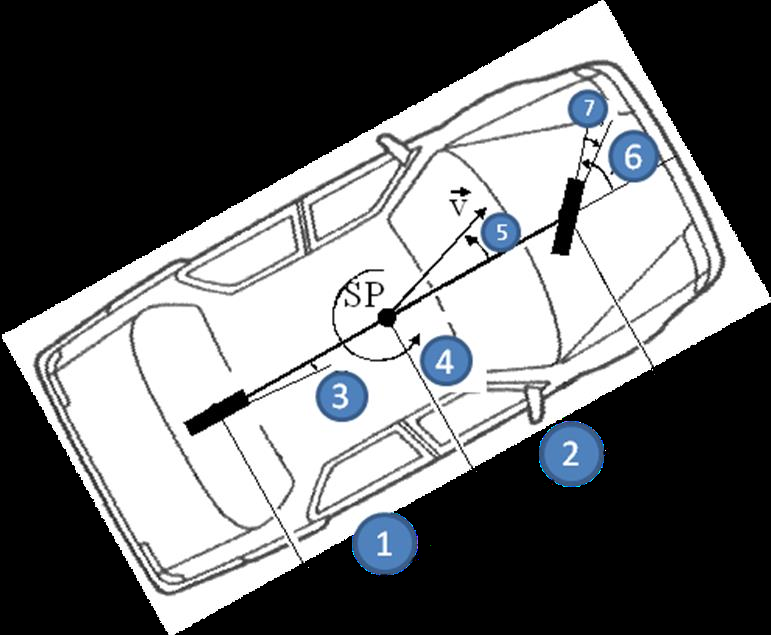
\includegraphics[width=\linewidth]{Graphics/Linearen_Einspurmodell.png}
    \end{minipage}
    \begin{minipage}[c]{.75\linewidth}
        \centering
        \begin{tabular}{|p{.05\linewidth}<{\centering}|p{.115\linewidth}<{\centering}|p{.75\linewidth}<{\centering}|}
            \hline
            Nr. & Bezeichnung & Bedeutung                        \\
            \hline
            1   & $l_H$       & Schwerpunktvorlage               \\
            \hline
            2   & $l_V$       & Schwerpunktr\"ucklage            \\
            \hline
            3   & $\alpha_H$  & Schräglaufwinkel von Hinterachse \\
            \hline
            4   & $\Psi$      & Gierwinkel                       \\
            \hline
            5   & $\beta$     & Schwimmwinkel                    \\
            \hline
            6   & $\delta$    & Lenkwinkel                       \\
            \hline
            7   & $\alpha_V$  & Schräglaufwinkel von Vorderachse \\
            \hline
        \end{tabular}
    \end{minipage}
\end{figure}
\subsection{Beobachter}
\subsubsection{}
\textbf{Wo liegen die Pole der Übertragungsmatrix eines Beobachters in Abhängigkeit von der Rückführungsmatrix L? Geben Sie eine Herleitung für Ihr Ergebnis an.}
\begin{equation}
    \begin{aligned}
        \dot{\hat{x}}               & =A\hat{x}+Bu+L(y-\hat{y})                          \\
        \hat{y}                     & =c\hat{x}                                          \\
        \dot{\hat{x}}               & =a\hat{x}+Bu+Ly-LC\hat{x}                          \\
                                    & =\left(A-LC\right)\hat{x}+Bu+Ly                    \\
        s\hat{X}                    & =\left(A-LC\right)\hat{X}+Bu+LY                    \\
        \left(sI-A+LC\right)\hat{X} & =Bu+LY                                             \\
        \hat{X}                     & =\textcolor{red}{\underbrace{\left(sI-A+LC\right)^{-1}}_{Polverteilung\ \ddot{U}bertragungsfunktion}}\left(Bu+LY\right) \\
    \end{aligned}
\end{equation}

\subsubsection{}
\textbf{Für folgendes System soll ein Beobachter zur Zustandsrekonstruktion so entworfen werden, dass die Beobachterfehlerdynamik einen doppelten Pol bei $s=-2$ aufweist.}

\begin{equation}
    \begin{array}{l}
        \dot{x}=\left[\begin{array}{cc}
                2  & 1 \\
                -1 & 0 \\
            \end{array}\right]x+\left[\begin{array}{c}
                0 \\
                1 \\
            \end{array}\right]u \\
        y=\left[1\qquad 0\right]x
    \end{array}
\end{equation}
\paragraph{1.Überprüfen Sie das System auf die Beobachtbarkeit.}

\

Kriterium:
\begin{equation}
    Q_B=\left[\begin{array}{c}
            C  \\
            CA \\
        \end{array}\right]\rightarrow\detmat\ Q_B\neq0
\end{equation}
\begin{equation}
    Q_B=\left[\begin{array}{cc}
            1 & 0 \\
            2 & 1 \\
        \end{array}\right]\rightarrow\detmat\ Q_B=1\rightarrow beobachtbar
\end{equation}
\paragraph{2. Bestimmen Sie die Beobachterkoeffizienten $l_1$ und $l_2$.}

\

\begin{equation}
    \detmat(sI-A+LC)=\left|\left[\begin{array}{cc}
            s-2+l_1 & -1 \\
            1+l_2   & s  \\
        \end{array}\right]\right|=s^2-2s+l_1s+1+l_2
\end{equation}
Weil die Beobachterfehlerdynamik einen doppelten Pol bei s = −2 aufweist, so die Koeffiziente proportional zu die von Gleichung $(s+2)(s+2)=0$ sein. Also:
\begin{equation}
    \begin{aligned}
        (s+2)(s+2)=\underbrace{s^2}+\underbrace{4s}+\underbrace{4}\  & \overset{Koeffizientenvergleichung}{\Longleftrightarrow}\ \underbrace{s^2}+\underbrace{(-2+l_1)s}+\underbrace{1+l_2} \\
                                                                     & \left\{\begin{array}{c}
            l_1=6 \\
            l_2=3 \\
        \end{array}\right.                                                                             \\
    \end{aligned}
\end{equation}